% Chapter 1

\chapter{Introduction} % Main chapter title

\label{Chapter1} % For referencing the chapter elsewhere, use \ref{Chapter1} 


\section{Motivation}

\xt{To be completed}

This research are trying to answer these questions.
\begin{itemize}
    \item How to implement offline program analysis for the ScaRR novel model for remote attestation?
    \item How is the performance of the analyzer?
    \item How is the performance comparison against some other attestation scheme such as C-Flat?
\end{itemize}

\section{Related Works}

\xt{Review the literature review here. Put sufficient figures.}

In this section we present related work in model for remote attestation. Specifically we discuss how different attestation scheme encode the offline program representations.

C-Flat \cite{aberaCFLATControlFlowAttestation2016} is the first remote attestation scheme to detect runtime control flow attack for embedded systems. C-Flat are generating offline measurement by traversing all possible path of program from start node to the termination node. In each node, C-Flat hashes the node ID and the hash of previous node. In the first node, since there is no previous hash, we pass 0. This creates hash chains which is stored as offline measurement database.

\begin{figure}[htbp]
\centerline{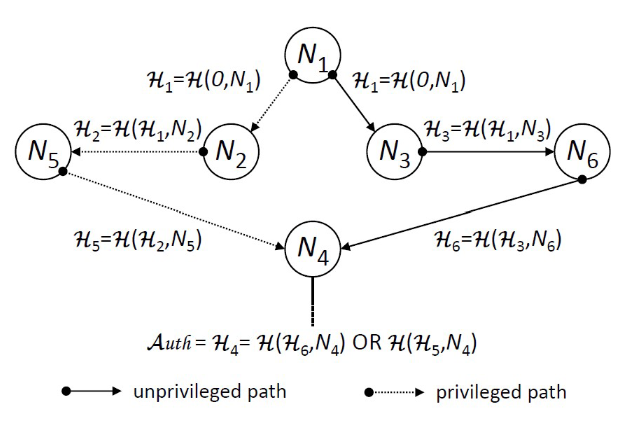
\includegraphics[scale=.5]{Figures/01/cflat.png}}
\caption{C-Flat. \ft{fix the figures. Put in sub-figure aside each other, if 
needed. Apply for all the figures in the thesis. Btw, you better redraw the 
figures from scratch, no crop from original paper :)}}
\label{fig:c-flat}
\end{figure}

Lo-Fat\cite{dessoukyLOFATLowOverheadControl2017} is improving C-Flat by using hardware support for control flow attestation. Lo-Fat offline program analysis is still inheriting C-Flat approach.

Atrium \cite{zeitouniATRIUMRuntimeAttestation2017} is remote attestation scheme that can provide resiliency against physical memory attack where adversaries can exploit the property of Time of Check Time of Use (TOCTOU) during attestation. In this paper author are describing memory bank attack where adversary can control instruction fetches to benign memory area when attestation is running and direct the fetch to the malicious area otherwise.

\begin{figure}[htbp]
\centerline{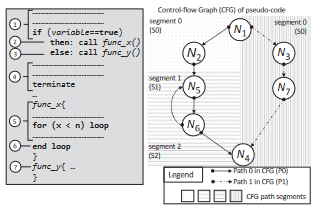
\includegraphics[scale=.5]{Figures/01/atrium.png}}
\caption{Atrium}
\label{fig:atrium}
\end{figure}

The offline measurement are calculated slightly different compared with C-Flat and Lo-Fat. In Atrium, the verifier perform one-time pre-processing to generate CFG of the program and computes cryptographic hash measurement over the instructions and addresses of basic blocks. C-Flat are only hash the node ID. While this approach can mitigate the TOCTOU attack, the offline measurement generation still grow exponentially as the complexity of the program grow. 

LiteHax \cite{dessoukyLiteHAXLightweightHardwareassisted2018} is hardware assisted remote attestation scheme that allow verifier to detect these different attacks:

\begin{itemize}
    \item control-data attack such as code injection or code reuse attack like ROP
    \item non-control-data attack
    \item data-only attack such us DOP which do not affect control flow
\end{itemize}

Different with the previous remote attestation scheme, the offline measurement phase of LiteHax are only generates program CFG without calculating any hash over all control flow and data flow events. However, in the online prover-side verification time, prover are still computing hash and sending it as report to the verifier. Verifier runs symbolic execution and incremental forward data-flow analysis without doing any lookup to offline measurement database.

Diat \cite{aberaDIATDataIntegrity2019} is remote attestation scheme that can attest data integrity and control-flow of autonomous systems. To improve efficiency of attestation, the program attested must be decomposed into small interacting modules. Data-flow monitoring is to be setup between critical modules. Control path attestation is being done against novel execution path representation using multiset has (MSH) function \cite{clarkeIncrementalMultisetHash2003}. The use of MSH makes some execution order of the program lost.

\begin{figure}[htbp]
\centerline{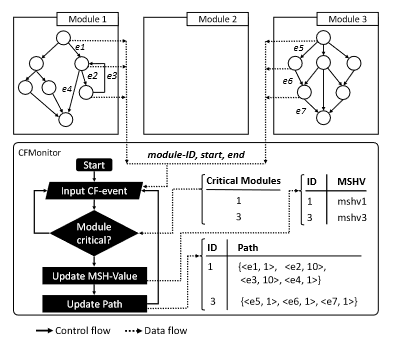
\includegraphics[scale=.5]{Figures/01/diat.png}}
\caption{Diat}
\label{fig:diat}
\end{figure}

OAT \cite{sunOATAttestingOperation2020} is remote attestation scheme to attest operation integrity of embedded device. OAT defines two type of measurements for control flow attestation: a trace (for recording branches and jumps) and a hash (for encoding returns). These two measurements are encoded as $H = Hash(H \bigoplus RetAddr)$ which called as attestation blob.

\begin{figure}[htbp]
\centerline{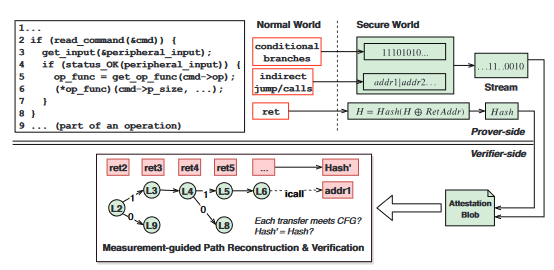
\includegraphics[scale=.5]{Figures/01/oat.png}}
\caption{OAT}
\label{fig:oat}
\end{figure}

During verification, verifier reconstruct paths from the attestation blob. The control flow violation is identified when CFI check against an address is failed or mismatched between hash and trace.

Although OAT does not encounter the combinatorial hash explosion in C-Flat, there is a verification overhead since verifier needs to reconstruct the attestation blob. TODO compare the overhead with ScaRR.
